\chapter{Downstream Polarimetry \& Magnetic Field Measurements}
\label{app:down_poldata}

\section{Downstream Polarimetry}

\begin{table}[h]
\centering
\begin{threeparttable}
\caption{List of cryomagnet settings used for the downstream neutron polarimetry.}
\label{tab:down_poldata}
\begin{tabular}{@{}lc@{}}
\toprule
Settings & Neutron/s/MW \\ \midrule
FCS\tnote{*}, MSE\tnote{**} & 2.73 $\pm$ 0.01 \\
FCS off, MSE off, flipper ON & 2.73 $\pm$ 0.01 \\
FCS off, MSE off & 2.73 $\pm$ 0.01 \\
FCS off, MSE off, flipper ON & 2.71 $\pm$ 0.01 \\
FCS off, MSE on & 3.09 $\pm$ 0.01 \\
FCS off, MSE on, flipper ON & 3.05 $\pm$ 0.01 \\
FCS off, MSE on & 3.03 $\pm$ 0.01 \\
FCS off, MSE on (large current) & 3.07 $\pm$ 0.02 \\
FCS on, MSE on (large current), degauss mu-metal coil & 2.99 $\pm$ 0.01 \\
FCS on, MSE on (large current), degauss mu-metal coil, degauss metglas coil & 3.02 $\pm$ 0.02 \\
FCS on, MSE off , degauss mu-metal coil, degauss metglas coil & 3.07 $\pm$ 0.02 \\
FCS on, MSE off , degauss mu-metal coil, degauss metglas coil & 3.10 $\pm$ 0.02 \\ \bottomrule
\end{tabular}

    \begin{tablenotes}
      \item[*] Earth’s Field Cancellation Coil
      \item[**] Magnetic Shield Enclosure Coil
    \end{tablenotes}

  \end{threeparttable}
\end{table}

\section{Magnetic Field Measurements}

\afterpage{
\begin{figure}
     \centering
     \begin{subfigure}[b]{0.75\textwidth}
         \centering
         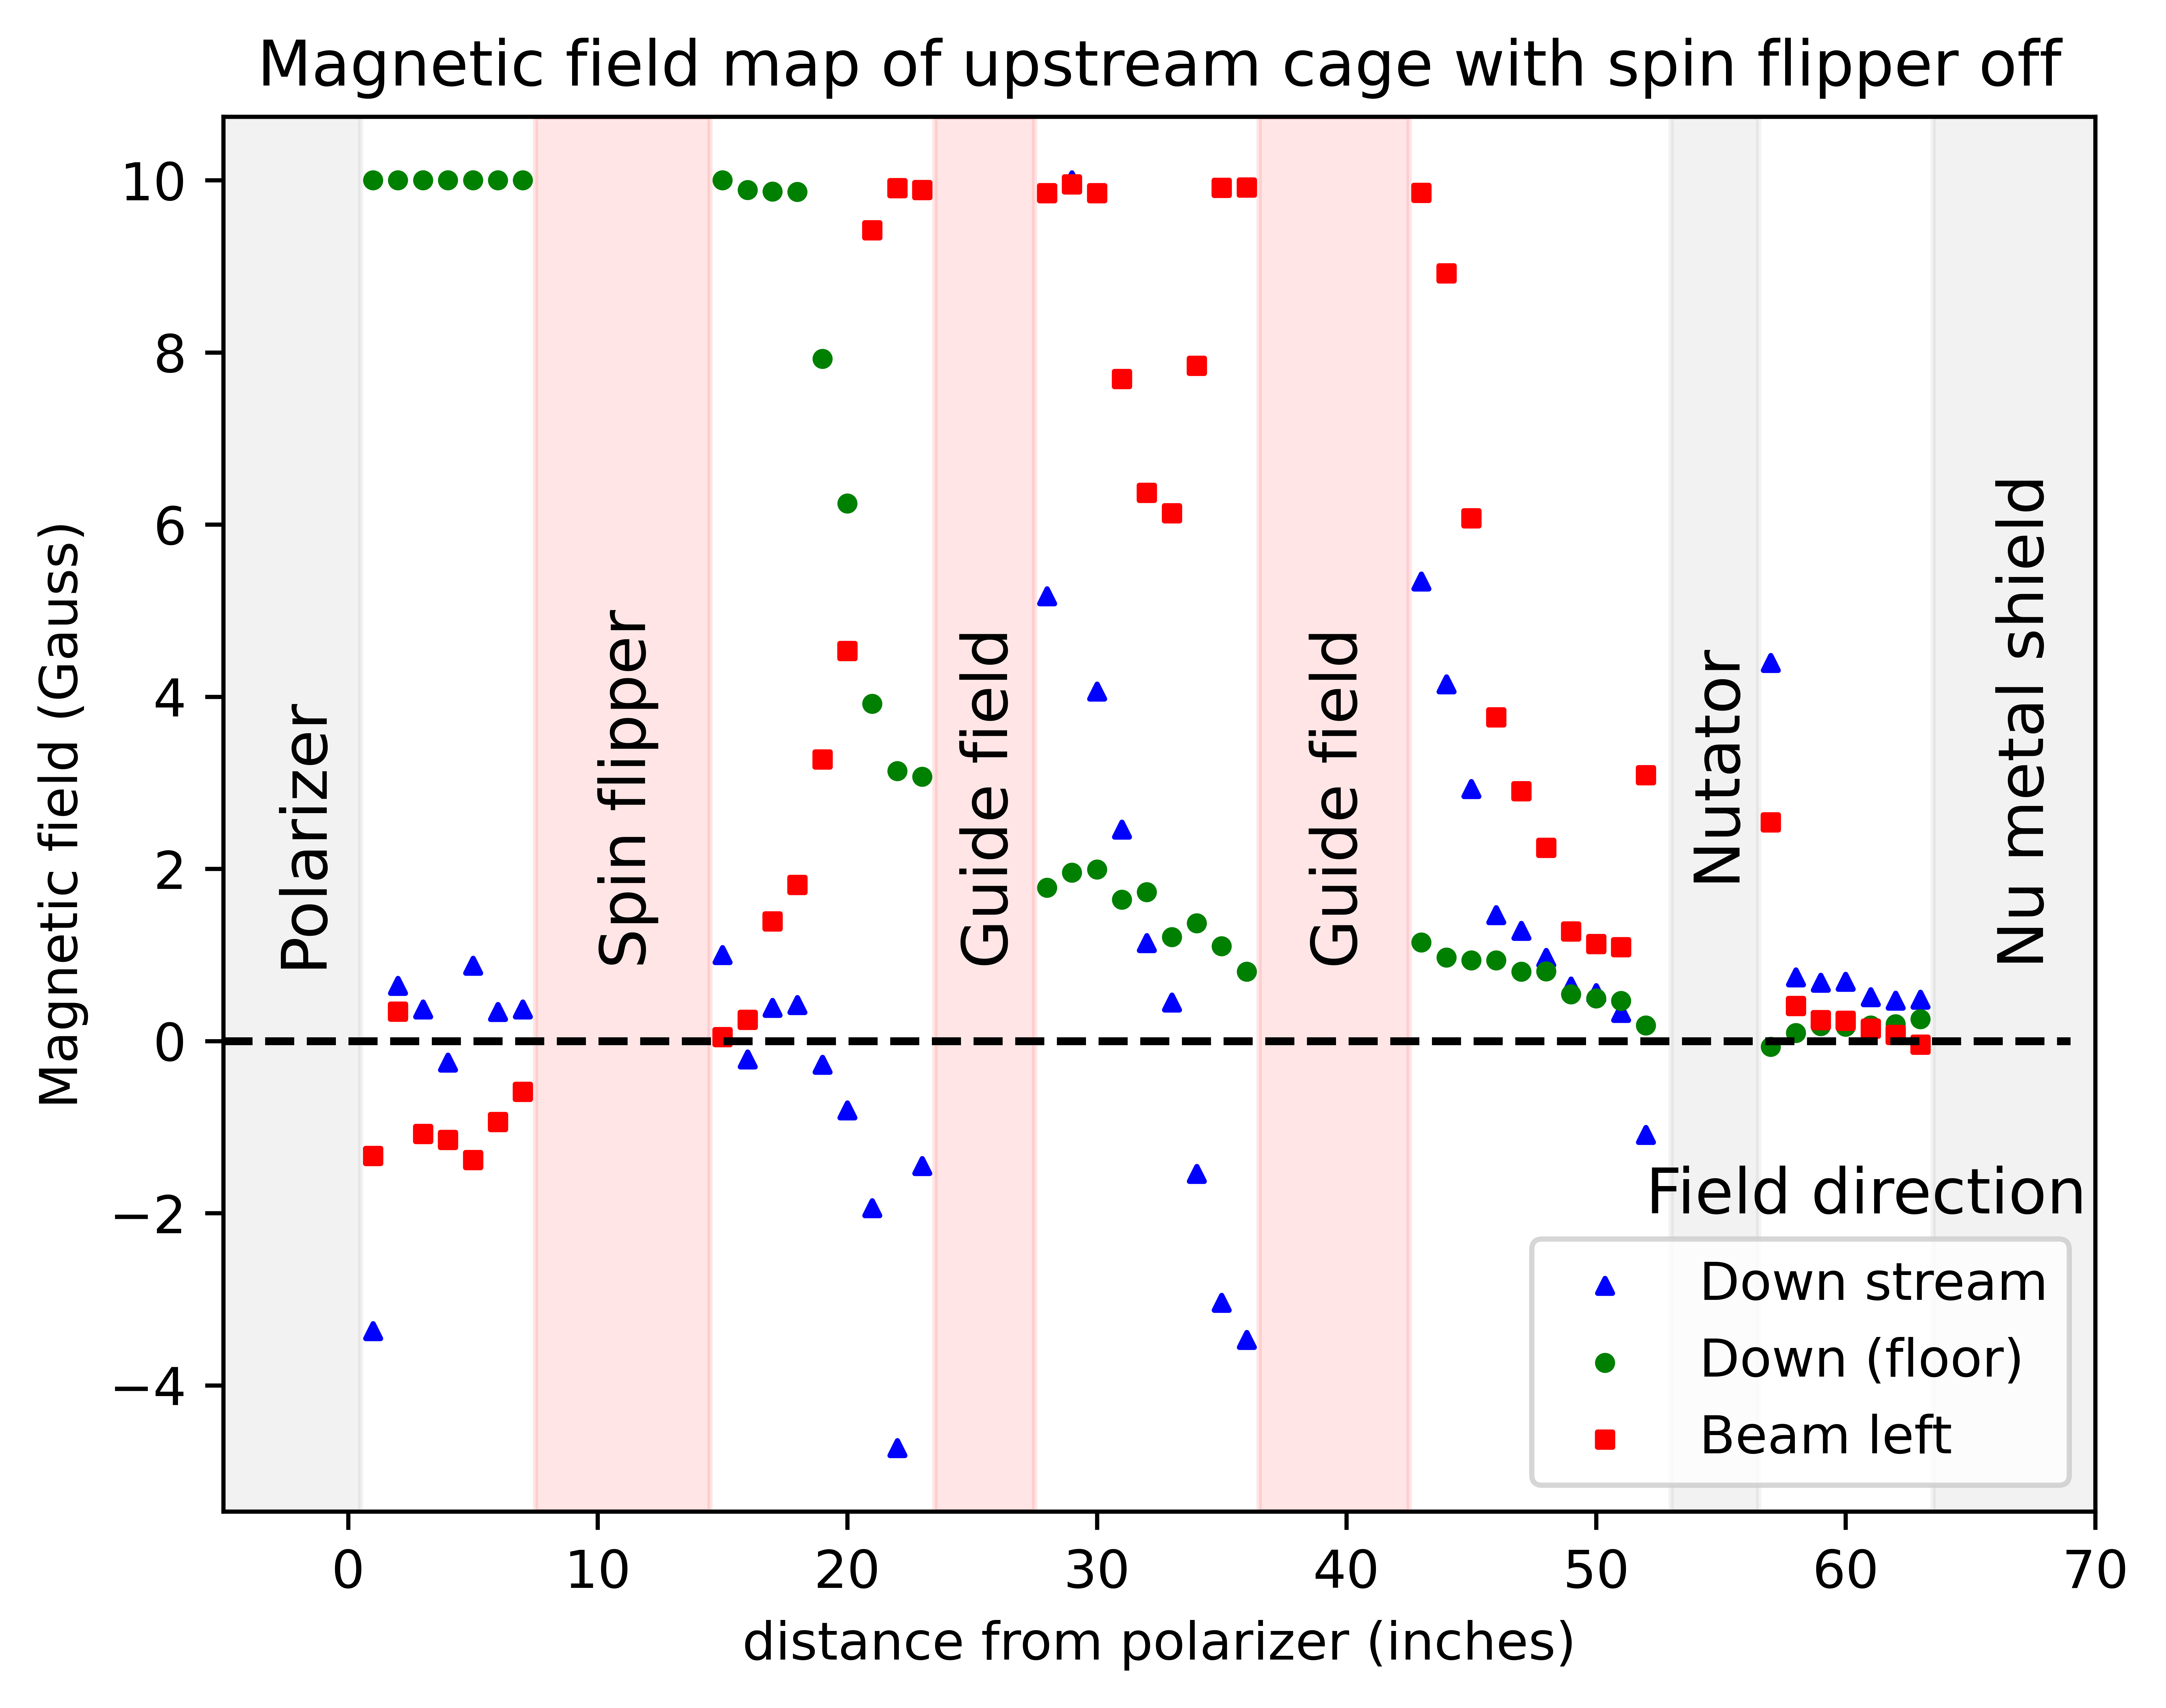
\includegraphics[width=\textwidth]{figures/appendix-figs/SpinOff.png}
         \caption{Upstream magnetic field profile.}
         \label{fig:up_mag}
     \end{subfigure}
     \hfill
     \begin{subfigure}[b]{0.75\textwidth}
         \centering
         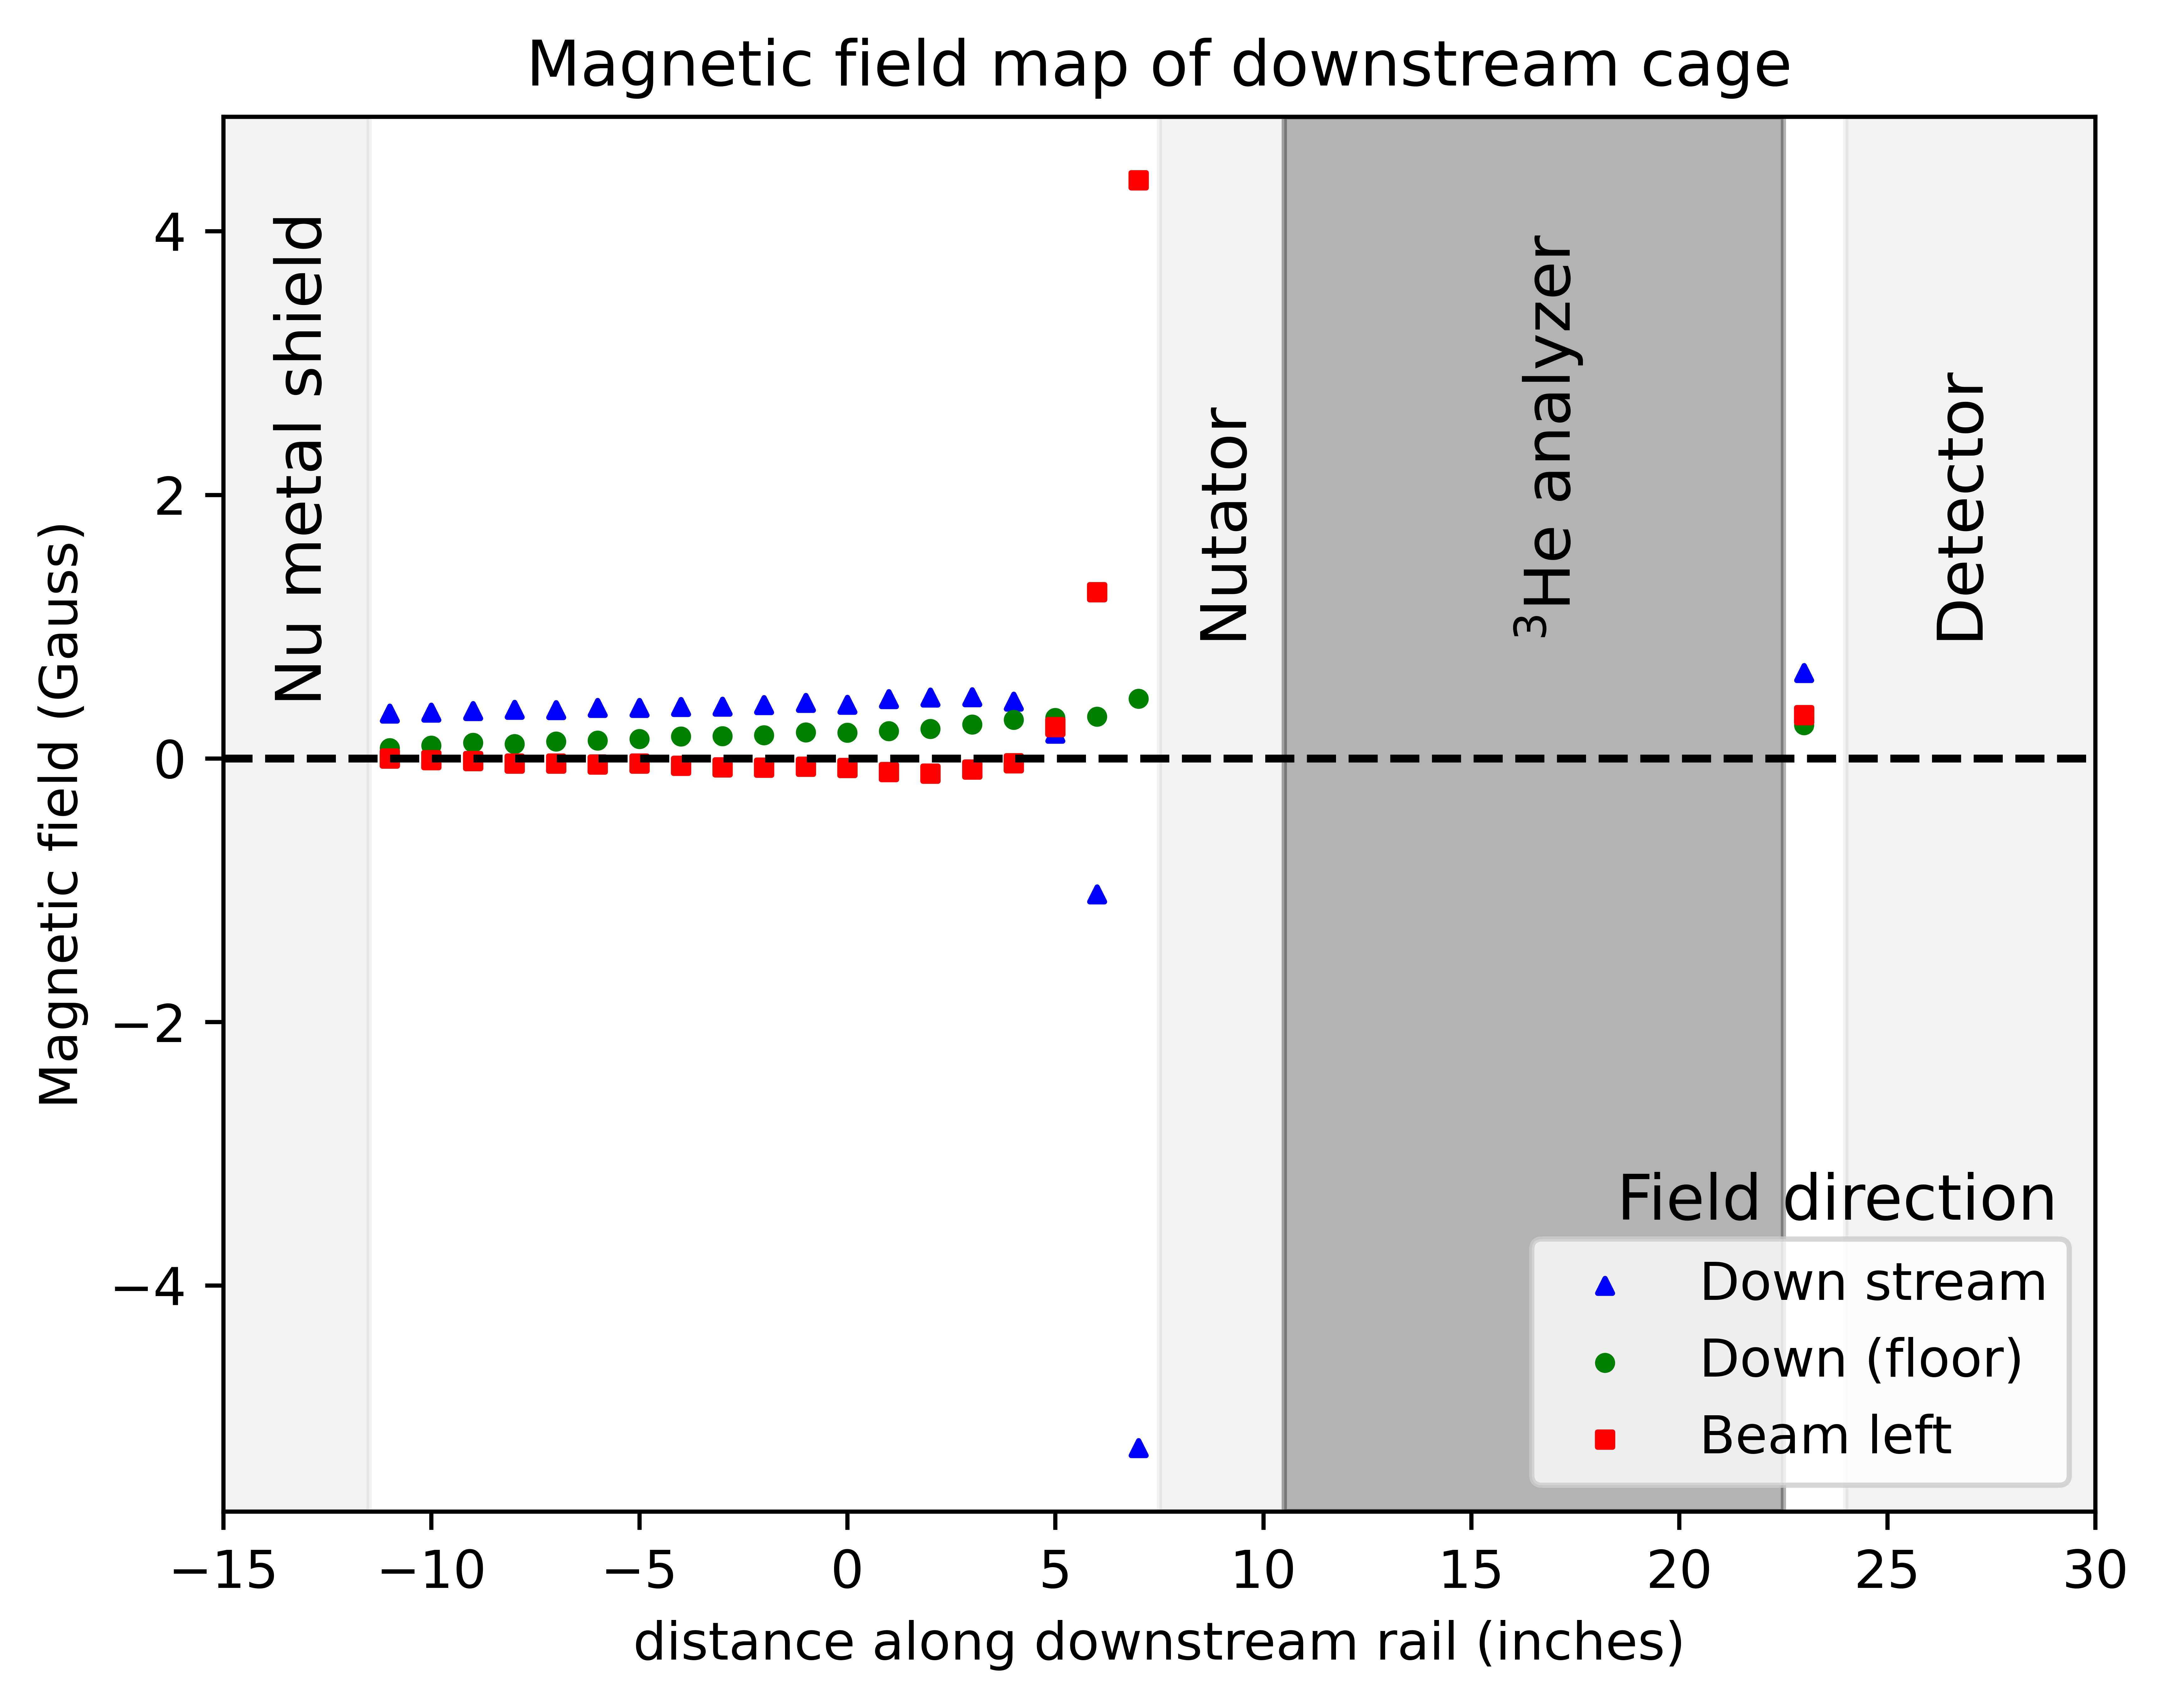
\includegraphics[width=\textwidth]{figures/appendix-figs/down.png}
         \caption{Upstream magnetic field profile.}
         \label{fig:down_mag}
     \end{subfigure}
        \caption{The magnetic field profile as measured along the neutron flight path.}
        \label{fig:measure_mag}
\end{figure}
\clearpage}